%%%%%%%%%%%%%%%%%%%%%%%%%%%%%%%%%%%%%%%%%
% Short Sectioned Assignment
% LaTeX Template
% Version 1.0 (5/5/12)
%
% This template has been downloaded from:
% http://www.LaTeXTemplates.com
%
% Original author:
% Frits Wenneker (http://www.howtotex.com)
%
% License:
% CC BY-NC-SA 3.0 (http://creativecommons.org/licenses/by-nc-sa/3.0/)
%
%%%%%%%%%%%%%%%%%%%%%%%%%%%%%%%%%%%%%%%%%

%----------------------------------------------------------------------------------------
%	PACKAGES AND OTHER DOCUMENT CONFIGURATIONS
%----------------------------------------------------------------------------------------

\documentclass[paper=a4, fontsize=11pt]{scrartcl} % A4 paper and 11pt font size

\usepackage[T1]{fontenc} % Use 8-bit encoding that has 256 glyphs
\usepackage{fourier} % Use the Adobe Utopia font for the document - comment this line to return to the LaTeX default
\usepackage[english]{babel} % English language/hyphenation
\usepackage{amsmath,amsfonts,amsthm} % Math packages

\usepackage{lipsum} % Used for inserting dummy 'Lorem ipsum' text into the template

\usepackage{sectsty} % Allows customizing section commands
\usepackage{graphicx}
\allsectionsfont{\centering \normalfont\scshape} % Make all sections centered, the default font and small caps

\usepackage{fancyhdr} % Custom headers and footers
\pagestyle{fancyplain} % Makes all pages in the document conform to the custom headers and footers
\fancyhead{} % No page header - if you want one, create it in the same way as the footers below
\fancyfoot[L]{} % Empty left footer
\fancyfoot[C]{} % Empty center footer
\fancyfoot[R]{\thepage} % Page numbering for right footer
\renewcommand{\headrulewidth}{0pt} % Remove header underlines
\renewcommand{\footrulewidth}{0pt} % Remove footer underlines
\setlength{\headheight}{13.6pt} % Customize the height of the header

\numberwithin{equation}{section} % Number equations within sections (i.e. 1.1, 1.2, 2.1, 2.2 instead of 1, 2, 3, 4)
\numberwithin{figure}{section} % Number figures within sections (i.e. 1.1, 1.2, 2.1, 2.2 instead of 1, 2, 3, 4)
\numberwithin{table}{section} % Number tables within sections (i.e. 1.1, 1.2, 2.1, 2.2 instead of 1, 2, 3, 4)

\setlength\parindent{0pt} % Removes all indentation from paragraphs - comment this line for an assignment with lots of text

\usepackage[T1]{fontenc}
\usepackage[utf8]{inputenc}
%----------------------------------------------------------------------------------------
%	TITLE SECTION
%----------------------------------------------------------------------------------------

\newcommand{\horrule}[1]{\rule{\linewidth}{#1}} % Create horizontal rule command with 1 argument of height

\title{}
\title{	
\normalfont \normalsize 
\textsc{Ecole Nationale des Ingénieurs de Brest} \\ [25pt] % Your university, school and/or department name(s)
\horrule{0.5pt} \\[0.4cm] % Thin top horizontal rule
\huge Ontologie de la notation musicale \\ % The assignment title
\horrule{2pt} \\[0.5cm] % Thick bottom horizontal rule
}

\author{Arthur Le Guennec \and Kwon-Young Choi}

\date{\normalsize\today} % Today's date or a custom date

\begin{document}

\maketitle % Print the title

%----------------------------------------------------------------------------------------
%	PROBLEM 1
%----------------------------------------------------------------------------------------

\section{Ontologie : définition}

Une ontologie est un ensemble structuré de terme et de relations permettant d'expliciter formellement les connaissances spécifiques lié à un domaine.
Les ontologies ont reçu beaucoup d'intérêt ces dernières années et il existe de nos jours énormément d'ontologie sur beaucoup de domaines variés.
En effet, lorsque une ontologie est créée pour décrire un domaine, cela permet de partager les connaissances du domaine entre humains mais aussi entre des agents virtuels.
Une ontologie est réutilisable et permet de séparer la connaissance liée spécifiquement à un domaine et la connaissance liée à l'implémentation pratique d'un logiciel ou d'un site web.
Enfin une ontologie permet aussi d'analyser les connaissances d'un domaine et donc de faire une sorte d'état de l'art du domaine.

Il existe plusieurs langages pour décrire une ontologie.
Dans le cadre du Web Sémantique, le W3C (World Wide Web Consortium) a énormément travaillé à développer et standardiser l'utilisation des ontologies.
Nous allons d'ailleurs utiliser ici le langage OWL (Web Ontology Language) qui s'appuie sur le standard RDF (Ressource Description Framework) et la syntaxe XML et qui a été spécifié par le W3C. 
Une ontologie est donc constituée de classes qui sont elle-même constituées de sous-classes.
Ces classes peuvent contenir des attributs qui permettent de décrire la classe.
Le plus intéressant étant le fait que l'on puisse faire des liens entre les classes avec des triplets RDF.

\section{Spécification d'une ontologie dans le cadre de la notation musicale}

\begin{figure}[btp]
  \centering
  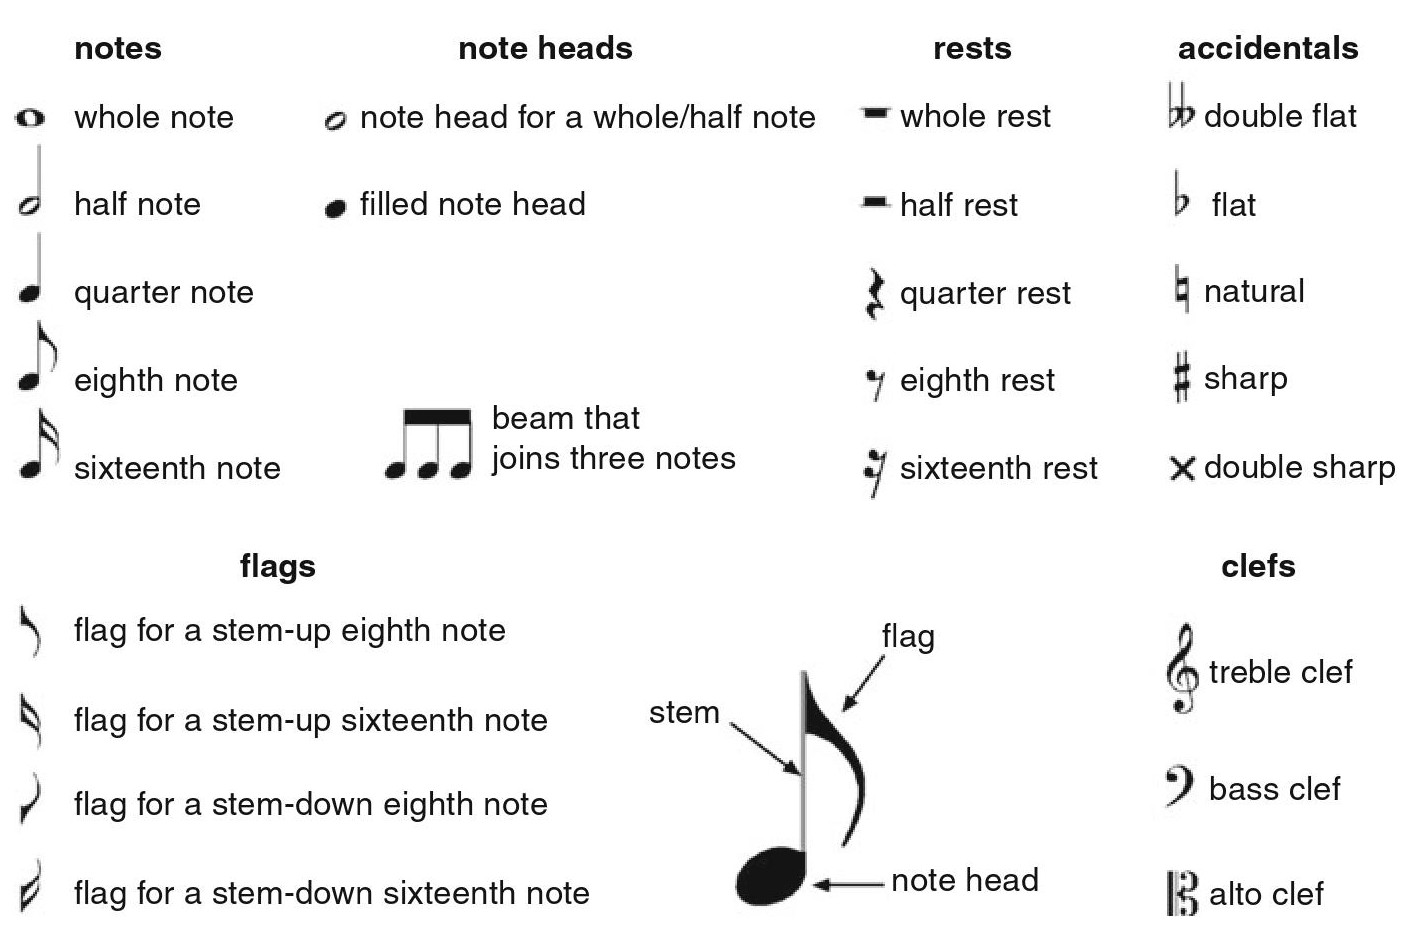
\includegraphics[scale=1]{list_symbols}
  \caption{\label{list_symbols} Liste des principaux symboles musicaux. }
\end{figure}

Une ontologie est utilisée pour expliciter les connaissances liées à un domaine spécifique.
Nous avons choisi ici de réaliser une ontologie pour expliciter la notation musicale.
La musique occidentale utilise une grammaire bidimensionnelle qui permet de décrire la hauteur, le rythme et le tempo d'une musique.
Cela permet la sauvegarde et le partage de la musique.

Une partition est donc un document utilisé pour formaliser la musique.
Son organisation est hiérarchique, par exemple :
\begin{itemize}
  \item Différentes portées sont utilisées pour différents instruments ou voix
  \item Chaque portée est divisé verticalement par cinq lignes
  \item Chaque portée est divisé horizontalement par des barres de mesures
  \item Chaque portée contient des symboles musicaux
\end{itemize}
Il existe de multiples symboles dans la notation musicale qui sont résumés dans la figure \ref{list_symbols} :
\begin{itemize}
  \item clefs
  \item notes
  \item silences
  \item altérations
  \item points
  \item \ldots
\end{itemize}

Durant ce travail, nous avons voulu représenter grâce à une ontologie l'organisation d'une partition musicale très simple.
Nous avons pris comme exemple de modéliser la partition de "J'ai du bon tabac dans ma tabatière".
Nous avons donc tout d'abord déclaré des classes de symboles comme les clefs qui contient des sous-classes qui représentent les différentes clefs utilisées dans la notation musicale comme la clef de sol.
La progression et le découpage du temps sont très important dans une partition.
Au début d'une partition, après la clef, on trouve la signature d'une partition définit par deux chiffres.
Le chiffre du bas indique la pulsation de base de la partition (quatre indique que la pulsation de base sera une noire (ou un quartet)) et le chiffre du haut indique combien de pulsations de base sont présentes dans une mesure.
On peut utiliser le caractère 'C' pour indiquer que la pulsation de base est de 4/4.
La durée d'une note est décris dans la notation musicale en utilisant des divisions.
En effet, si l'on considère que la durée d'une ronde est de 1, la durée d'une blanche sera donc de 1/2, la durée d'une noire de 1/4 et la durée d'une croche de 1/8, \ldots
Enfin, la hauteur ou fréquence d'une note est décris dans la classe pitch et qui contient les sept notes : Do, Ré, Mi, Fa, Sol, La, Si (ou C, D, E, F, G, A, B dans la notation anglo-saxonne).
Ces notes peuvent être augmentées d'un demi-ton en ajoutant une altération comme un dièse à côté de la note.
Une autre utilisation des altérations est de les mettre en début de portées et dire qu'une note est altérée d'un demi-ton pour toute la durée de la partition.

C'est donc dans la classe Music Score que contient vraiment la partition de "J'ai du bon tabac dans ma tabatière".
Cette classe contient donc des attributs comme le titre, mais aussi des relations comme le fait que pour toute la partition, la note Fa sera augmenté d'un demi-ton, la clef de la partition est la clef de Sol et que la signature temporelle de la partition est de 4/4.
Des sous-classes mesures définissent les mesures contenu dans la partition.
Chaque mesure est suffixée d'un nombre que qui permet de modéliser la progression du temps.
Ce même système est utilisé pour la progression des notes contenues dans les mesures.
Une note est une sous-classe d'une mesure et contient les attributs de hauteur et de durée.


%\bibliographystyle{plain}
%\bibliography{hmm}

\end{document}
